\clearpage

\begin{figure}[h]
\caption{Mindfulness of Breathing (\emph{Ānāpānasati})}\label{fig-mindfulness-of-breathing}
\bigskip\centering
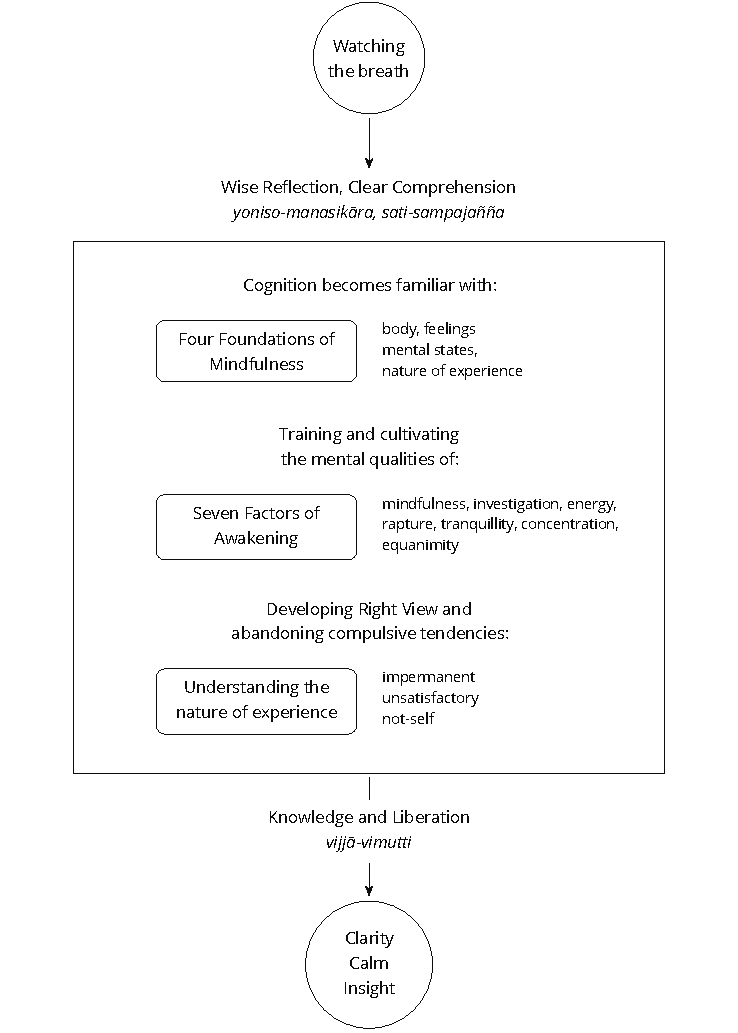
\includegraphics[scale=0.8]{mindfulness-of-breathing.pdf}
\par
\end{figure}

\clearpage

\section{Mindfulness of Breathing (excerpt)}

{\centering
\emph{\href{https://suttacentral.net/mn118}{MN 118}, Ānāpānasati Sutta}
\par}

{
\setlength{\parindent}{0pt}\setlength{\parskip}{5pt}
\fontsize{9.5}{14}\selectfont

Bhikkhus, when mindfulness of breathing is developed and cultivated, it is of great fruit and great benefit.
When mindfulness of breathing is developed and cultivated, it fulfills the Four Foundations of Mindfulness.
When the Four Foundations of Mindfulness are developed and cultivated, they fulfill the Seven Factors of Awakening.
When the Seven Factors of Awakening are developed and cultivated, they fulfill true knowledge and deliverance.

And how, bhikkhus, is mindfulness of breathing developed and cultivated, so that it is of great fruit and great benefit?

Here, bhikkhus, a bhikkhu, gone to the forest, to the foot of a tree or to an
empty hut, sits down having crossed his legs, sets his body erect, having
established mindfulness in front of him.

Ever mindful he breathes in; mindful he breathes out.

\textbf{Body}

Breathing in \& out long, he knows:\\ `I breathe in \& out long';

Breathing in \& out short, he knows:\\ `I breathe in \& out short';

He trains thus:\\ `I shall breathe in \& out experiencing the whole body'.

He trains thus:\\ `I shall breathe in \& out tranquillizing the bodily formations'.

\clearpage

\textbf{Feelings}

He trains thus:

`I shall breathe in \& out experiencing rapture'.

`I shall breathe in \& out experiencing pleasure'.

`I shall breathe in \& out experiencing the mental formations'.

`I shall breathe in \& out tranquillizing the mental formations'.

\textbf{Mental States}

He trains thus:

`I shall breathe in \& out experiencing the mind'.

`I shall breathe in \& out gladdening the mind'.

`I shall breathe in \& out concentrating the mind'

`I shall breathe in \& out liberating the mind'.

\textbf{Nature of Experience}

He trains thus:

`I shall breathe in \& out contemplating impermanence'.

`I shall breathe in \& out contemplating the fading away of passions'.

`I shall breathe in \& out contemplating cessation'.

`I shall breathe in \& out contemplating relinquishment'.

\bigskip

Bhikkhus, that is how mindfulness of breathing is developed and cultivated, so that it is of great fruit and great benefit.

}
